\chapter{Backend}

\section{Kommunikation}

\subsection{Zeitkritische Informationen}
Als zeitkritisch werden Informationen eingestuft, sofern sie die direkten Eingaben der ControlClients und eventuelles Feedback des OutputClient betreffen. Da es sich um ein Reaktionsspiel handel,t müssen diese Daten zeitnah von Sender zu Empfänger gelangen. Solch eine Relation ist nur über eine Peer-to-Peer Verbindung zu realisieren.

\subsection{Möglichkeit 1: Predefined Packages 'rtc.io'}
Der NodeJS Server wird als Verbindungsserver für die Etablierung einer Peer-to-Peer Verbindung zwischen ControlClients und OutputClient genutzt. Als Technik wird konret WebRTC eingesetzt. Auf dem NodeJS-Server wir das Package "rtc-switchboard" eingesetzt, welches eine Grundlage für einen  Signalisierungsserver ist. Die Clients nutzen "rtc-quickconnect" um neues Channels anzufordern und eine Peer-to-Peer Verbindung zu etablieren.



\subsubsection{Vorteile}
\begin{itemize}
\item
Leichtere Implementierung, da alle Ebenen der Kommunikation bereits abgedeckt wurden und nur noch semantisch auf Informationen eingegangen werden muss.
\end{itemize}

\subsubsection{Nachteile}
\begin{itemize}
\item
Durch Generalisierung ein deutlicher Overhead.

\item
Status ist offiziell noch 'unstable'.
\end{itemize}

\subsection{Möglichkeit 2: Abstrakte WebRTC implementation 'WebRTC'}
Wie auch bei Möglichkeit 1 wird der NodeJS-Server als Verbindungsserver genutzt. Jedoch muss auf Client-Seite, also für OutputClient und ControlClient, eine eigene Signalling Implementation stattfinden. Es wird eine viel abtraktere Schicht genutzt.


\subsubsection{Vorteile}
\begin{itemize}
\item
Da die genutzen Packages nur eine Grundlage bilden, ist eine spezialisierte Implementierung möglich.
\end{itemize}

\subsubsection{Nachteile}
\begin{itemize}
\item
Implementierungsaufwand deutlich höher.

\item
Spezialisierung für dieses Projekt eventuell nicht nötig.

\item
Status ist offiziell noch 'unstable'.
\end{itemize}

\subsection{Möglichkeit 3: Socket.io P2P}
Das Package Socket.io bietet auch selber eine Peer-to-Peer lösung auf WebRTC Basis. Hierbei wird eine Spezielle Art eines Sockets genutzt, welche wie ein normaler WebSocket agiert, bis ein Upgrade durchgeführt wird und die Clients nun direkt miteinander Kommunizieren.


\subsubsection{Vorteile}
\begin{itemize}
\item
Das Signalling und die P2P Kommunikation können mit einem Package geregelt werden.

\item
Variabel kann die Kommunikation über den Server, oder P2P ablaufen.

\item
Signalling events werden von Client-Server Kommunikation direkt zu P2P übernommen.
\end{itemize}

\subsubsection{Nachteile}
\begin{itemize}
\item
Wenig Einfluss auf die Upgrade-Mechanismen.
\end{itemize}

\subsection{Statusinformationen}
Für den Austausch nicht zeitkritischer Statusinformationen werden zwischen den Clienten und dem Server einfache WebSockets verwendet. Der Austausch von Zeitkritischen Statusinformationen muss über das Signalling des WebRTC durchgeführt werden.

\subsection{Fazit}
Die eigene Implementation auf Basis des WebRTC bietet die meisten Möglichkeiten, birgt jedoch auch enorme Risiken. RTC.io bietet eine Implementation die sehr gut für Prototypen geeignet ist, aber neben dem Zeitunkritischen Signalling eine eigene Einheit bietet, welche eine Generalisierung des WebRTC darstellt und somit viel Overhead besitzt. Die P2PImeplementierung von Socket.io steht von der Implementierungs Komplexität in der Mitte. Es bietet viele bereits bekannte Mechanismen des Client-Server Signalling über Events, welche mit einem Upgrade nun auch von Client zu Client funktionieren. 

Socket.io P2P entspricht den Anforderungen und wird für den Prototypen verwendet.

\subsection{Fazit nach Test}
Nach und auch schon während der Entwicklung des Prototypen hat sich rausgestellt, dass Socket.io P2P in der Implementierung viele Fehler aufweist. Eine teilweise Abänderung des Moduls führt näher an das gewünschte Ergebnis, verursacht aber intern wieder mehr Fehler als eigentlich gelöst wurden.

Socket.io P2P entspricht den Anforderungen, weißt aber zu große Mängel auf. Ein eigenes Modul, welches für unsere Anforderungen speziell entwickelt wird soll nun diesen Platz einnehmen.

\section{Eigenes Modul Kommunikation}
\subsection{Anforderungen an das eigene Modul für WebRTC}
\begin{itemize}
\item 
Es muss möglich sein, unsere ControlPeers nur mit dem DisplayPeer zu verbinden, nicht aber untereinander.

\item
Der DisplayPeer muss zu jedem ihm zugeordneten ControlPeer verbunden sein.

\item
Es Muss auf Serverseite eine Raumlogik existieren, um die Peers zuordnen zu können.

\item
Das Signalling muss weiterhin über den Server stattfinden.
\end{itemize}

\subsection{Zuweisungslogik Server}
Der Server hat bezüglich der Zuweisungen für Verbindungen die Aufgabe alle Clients zu gruppieren. Dies soll ähnlich wie bei Socket.io über eine Raumlogik geschehen. Es existieren Räume, in welche die Sockets auf dem Server (je Client also einer) eingeordnet werden.


Hierbei unterscheiden sich die Clients in ihrem Kommunikationsmodus:
\begin{description}
\item[Single]
Ein Client mit dem "Single" Modus pflegt nur eine direkte WebRTC Verbindung.

\item[Multi]
Ein Client mit dem "Multi" Modus pflegt mehrere direkte WebRTC Vebindungen gleichzeitig und agiert zwischen den ganzen Peers als "Host".
\end{description}

\begin{figure}[ht]
\centering
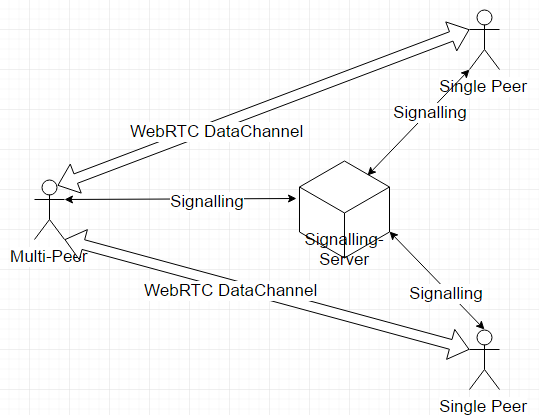
\includegraphics[width=0.9\textwidth]{backend/ConnectionBetweenPeers.PNG}
\caption{Verbindungsnetz}
\label{backfig1}
\end{figure}

In Abbildung \ref{backfig1} ist zu sehen, wie ein "Multi-Peer" mit mehreren "Single-Peer" gleichzeitig über WebRTC (konkret den DataChannel) kommuniziert, jeder einzelne "Single-Peer" aber nur mit dem einen "Multi-Peer". Zu sehen ist außerdem, dass das Signalling weiterhin für alle Peers über den Signalling-Server stattfindet, welcher hier auch gleichzeitig der WebServer ist.

\subsection{Zuweisungslogik Client (Single)}
Von nun an wird der Client der den Single Modus nutzt als "Single-Peer" bezeichnet.


Der Single-Peer pflegt nur eine WebRTC Verbindung, somit muss keine Zuweisungslogik geschehen.

\subsection{Zuweisungslogik Client (Multi)}
Von nun an wird der Client der den Multi Modus nutzt als "Multi-Peer" bezeichnet.


Der Multi-Peer pflegt mehrere WebRTC Verbindungen zu verschiedenen Single-Peers. Identifiziert werden die einzelnen Single-Peers über ein vom Server beim Signalling gesetztes Attribut in den Signalling Nachrichten: "from". Über dieses Attribut weiß der Multi-Peer von wem diese Signalling-Message kommt und kann so alle ankommenden Informationen diesem Single-Peer zuordnen. Somit wird unter dem alias des Single-Peer ein eigenes "webRTCConnection"-Objekt verwaltet/abgelegt.

\subsection{Identifizierung der Peers}
Die Peers selber erhalten in allen Signalling-Messages ein Attribut, über welches sie den Ursprung ermitteln können, um so Signale Peers zuordnen zu können. Diese "ID" wird vom Server vergeben und entspricht einfach nur der Socket ID welche die einzelnen Clients in Verbindung zum Server haben.

\section{Signalling Ablauf}
Der Ablauf ist bei den Single-Peers, sowie bei den Multi-Peers nahezu gleich.

\subsection{Anmeldung beim Server}
\begin{description}
\item[Multi-Peer]
Der Multi-Peer meldet sich beim Server mit der Bitte einen Raum zu erstellen. Sollte dieser Raum schon existieren ist dies ein Fehler, da in jedem Raum nur ein Multi-Peer existieren darf. Sollte der Raum noch nicht existieren, wird er erstellt und der Multi-Peer diesem zugewiesen.

\item[Single-Peer]
Der Single-Peer meldet sich beim Server mit der Bitte einen Raum zu betreten. Sollte dieser Raum noch nicht existieren ist dies ein Fehler, da ein Raum in diesem Projekt ein Spiel darstellt, ein Single-Peer (Control-Peer) aber nur einem bestehenden Spiel beitreten kann. Sollte der Raum bereits existieren und alle weiteren Spielablaufrelevanten Informationen stimmen (das Spiel darf zum Beispiel noch nicht angefangen haben), so tritt der Single-Peer diesem Raum bei. Direkt nach dem Beitreten eines Raumes, wird eine Signal an den Server gesendet, dass wir da sind.

\item[Server]
Sobald ein Raum existiert und ein Multi-Peer diesem zugewiesen ist, sendet jeder neu dazukommende Single-Peer ein Signal an den Server, dass er da ist. Dieses Signal wird nur an den Multi-Peer weitergeleitet.
\end{description}

\subsection{Erstes Signal}
\begin{description}
\item[Multi-Peer]
Jedes mal, wenn der Multi-Peer ein neues erstes Signal eines Single-Peers über den Server erhält ("hereandready"), ermittelt er seine ICE-Candidates und sendet diese an den Signalisierenden Single-Peer.
\end{description}

\subsection{ICE Candidates}
\begin{description}
\item[Multi-Peer]
Erhält ein Multi-Peer einen ICE-Candidate wird dieser der Passenden Verbindung hinzugefügt und löst das "negotationneeded"-Event aus, welches ein neues Offer in Form von SDP Signalisiert.

\item[Single-Peer]
Erhält ein Single-Peer einen ICE-Candidate wird dieser der akutellen webRTCCOnnection hinzugefügt und löst das "negotationneeded"-Event, welches ein neues Offer in Form von SDP Signalisiert.
\end{description}

\subsection{Aufbau über SDP}
\begin{description}
\item[Multi-Peer]
Erhält der Multi-Peer ein Offer in Form von SDP erwiedert er dieses mit einer Answer auch in Form von SDP und fügt die "remoteDescription" dieser WebRTCConnection auf Basis der Offer hinzu. Sofern dieser Vorgang erfolg hatte ist eine direkte Verbindung zwischen Multi-Peer und Single-Peer entstanden.

\item[Single-Peer]
Erhält der Multi-Peer ein Offer in Form von SDP erwiedert er dieses mit einer Answer auch in Form von SDP und fügt die "remoteDescription" dieser WebRTCConnection auf Basis der Offer hinzu. Sofern dieser Vorgang erfolg hatte ist eine direkte Verbindung zwischen Multi-Peer und Single-Peer entstanden.
\end{description}

\subsubsection{Kommunikationskanal}
Da es sich um einfache Steuerungsdaten handelt verwenden beide Modi der Peers einen simplen DataChannel.

\section{Eigenes Modul Aufbau}
\subsection{Schnittstelle}
\begin{figure}[ht]
\centering
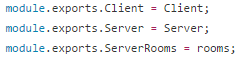
\includegraphics[width=0.9\textwidth]{backend/ModulExports.PNG}
\caption{Modul Exporte}
\label{backfig2}
\end{figure}

\begin{description}
\item[Modul.Client]
Unter Modul.Client ist eine Klassenorientierte Repräsentation des Clients zu finden. Es ist ein Object dieses Typs zu erzeugen.

\item[Modul.Server]
Unter Modul.Server ist eine Repräsentation des Servers zu finden. Für jeden auf dem Server neu Verbundenen Client muss eine neue (anonyme) Instanz dieses Typs erstellt und dabei der Socket der mit dem Client verbunden ist übergeben werden.

\item[Modul.ServerRooms]
Unter Modul.ServerRooms ist eine Simple Liste der derzeitigen Räume auf dem Server, inklusive der darin befindlichen Clients zu sehen. Diese Informationen sind jedoch nur auf Serverseite bei Verwendung des Modul.Server einsichtlich, bzw. werden nur unter Verwendung von Modul.Server aktualisiert.
\end{description}

\subsection{Abhängigkeiten}
Das Modul ist derzeit direkt von Socket.io abhängig, von welchem es die WebSockets für das Signalisierungen über den Signalling-Server nutzt.

\subsection{Struktur}
Das Modul implementiert zwei Teile. Erstens die Client-Seite. Zweitens die Server-Seite.

\subsubsection{Client}
Die Client-Implementation ist für das Frontend gedacht und nutzt alle WebRTC Standarts des webkit. Es handelt alle Faktoren von Initiierung der Kommunikation, bis Durchführung dieser ab.

\subsubsection{Server}
Die Server-Implementation kümmert sich auf Server-Seite um die Einhaltung von Kommunikations-Standarts, die Zuweisung von Signalen und die Gruppierung vieler Peers.